\chapter{Creating geometric elements}
\label{ch:create}
After having initialized the drawing panel as described in the previous Chapter, %~\ref{ch:start},
the next step is to create geometric elements in the drawing panel.

Remember, we have initialized the drawing panel similar to the following code.
\begin{lstlisting}[language=HTML]
<script type="text/javascript">
 var board = JXG.JSXGraph.initBoard('box', 
            {boundingbox:[-5,5,5,-5], axis:true});
</script>
\end{lstlisting}
Through the JavaScript variable \lstinline|board| in the above listing we have access to the drawing panel 
and can place objects there. New geometry elements can be added to the board. 
All elements are added with the method \lstinline|board.create()|. One example:
\begin{lstlisting}
board.create('point', 
        [1,3], 
        {name:'A', strokecolor:'red'}
        );
\end{lstlisting}
Another example:
\begin{lstlisting}
board.create('point', 
        [function(){return s.X();},function(){return t.X()}], 
        {trace:true}
        );
\end{lstlisting}
The parameters of the method \lstinline|board.create()| are:
\begin{lstlisting}
board.create(elementType, parents, attributes);
\end{lstlisting}
where
\begin{itemize}
    \item \lstinline|elementType| is a string containing the type of the element which is constructed. 
       At the moment, possible types are:
        \begin{itemize}
          \item primitive elements like points, lines, curves
          \item composite elements like bisectors, midpoints 
        \end{itemize}
    \item \lstinline|parents| is an array containing the parameters which define the element. 
    This can be parent elements like two points which define a line. It can also consist of JavaScript functions, numbers, and strings containing \geonext{}\sidenote{see http://geonext.de} syntax. The possible array elements depend on the element type.
    \item \lstinline|attributes| is an optional argument and has to be a JavaScript object. 
    Usually it is given in the form 
    \lstinline|{key1:value1, key2:value2, ...}|, called the ``literal object'' form.
\end{itemize}



Through the variable \lstinline|board| new geometry elements can be added to the board. All elements are added with the method \lstinline|board.create()|: 
\begin{lstlisting}
board.create('point', [1,3], {name:'A', strokecolor:'red'});
\end{lstlisting}

Another example: 
\begin{lstlisting}
board.create('point', [function(){return s.X();},function(){return t.X()}], {trace:true});
\end{lstlisting}

The parameters of \lstinline|board.create()| are: 
\begin{lstlisting}
board.create(elementType, parentElements, attributes);
\end{lstlisting}

\begin{lstlisting}
{key1:value1, key2:value2, ...}
\end{lstlisting}

Point is an easy example.

    * Properties of a point:
          o style
          o strokeColor
          o strokeWidth
          o fillColor
          o highlightStrokeColor
          o highlightFillColor
          o labelColor
          o visible
          o fixed
          o draft
          o trace 
    * Additional properties of a line:
          o straightFirst
          o straightLast 

There are no additional properties of a circle

    * Additional properties for an element:
          o needsRegularUpdate = [true]/false (eg axis are set to needsRegularUpdate=false) These elements are updated only, if the origin of the board is moved or after zooming 
    * Possible parameters: 

\begin{lstlisting}
el.setProperty('key1:value1','key2:value2',...);
el.setProperty([key1:value1],[key2:value2],...);
el.setProperty({key1:value1, key2:value2},...);
\end{lstlisting}

\subsection{Construction of a free point}
This example in Figure~\ref{fig:2} shows how to construct a simple, draggable point. 
\begin{figure*}[htb]
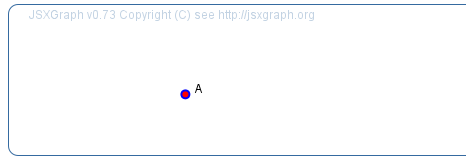
\includegraphics[width=0.4\linewidth]{images/b3.png}
\caption{The first JSXGraph point.}\label{fig:2}
\end{figure*}

\noindent It is produced by the following commands:
\begin{lstlisting}[language=html]
<div id="box" class="jxgbox" 
    style="width:200px; height:200px;"></div>
<script type="text/javascript">
 var board = JXG.JSXGraph.initBoard('box', 
                {boundingbox:[-2,2,2,-2]});
 var p = board.create('point',[0,1]);
</script>
\end{lstlisting}

The JavaScript code has to be placed {\sl after} the div element which will contain the construction. From now on, we will only show the JavaScript code. 

\subsection{Attributes of a point}
Several attributes can be given to change the properties of a point, for example a name or the point style. 
\begin{lstlisting}
 var board = JXG.JSXGraph.initBoard('box', 
                {boundingbox:[-2,2,2,-2]});
 var p = board.create('point',[0,1],{name:'X',face:'[]',size:4});
\end{lstlisting}
The resulting point in Figure~\ref{fig:3} is now labeled with ``X'' and is display as square with side length 4 pixel.
\begin{figure*}[htb]
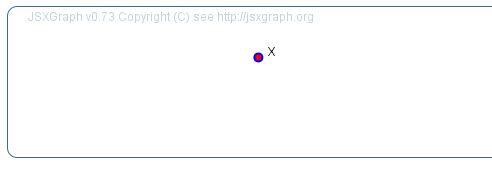
\includegraphics[width=0.4\linewidth]{images/b4.png}
\caption{The JSXGraph point ``X''.}\label{fig:3}
\end{figure*}

\paragraph{Point styles}
The layout of a point can be influenced by the property \lstinline|type|. It can attain the values $0,1,\ldots,12$. 
Alternatively of these equivalent constants can be used:

\bigskip
\begin{center}
\footnotesize
\begin{tabular}{lll}
\toprule
Constant &    value   & description \\
\midrule
\lstinline|JXG.POINT_STYLE_X_SMALL| &     0  & Small x \\
\lstinline|JXG.POINT_STYLE_X|  & 1&   Medium x \\
\lstinline|JXG.POINT_STYLE_X_BIG|  & 2  & Big x \\
\lstinline|JXG.POINT_STYLE_CIRCLE_TINY|  &   3 &  Tiny circle \\
\lstinline|JXG.POINT_STYLE_CIRCLE_SMALL|  &  4  & Small circle \\
\lstinline|JXG.POINT_STYLE_CIRCLE| & 5 &  Medium circle \\
\lstinline|JXG.POINT_STYLE_CIRCLE_BIG| & 6  & Big circle \\
\lstinline|JXG.POINT_STYLE_SQUARE_SMALL|&   7&   Small square \\
\lstinline|JXG.POINT_STYLE_SQUARE|&  8  & Medium square \\
\lstinline|JXG.POINT_STYLE_SQUARE_BIG|&  9 &  Big square \\
\lstinline|JXG.POINT_STYLE_PLUS_SMALL|&  10 & Small $+$ \\
\lstinline|JXG.POINT_STYLE_PLUS|&   11  &Medium $+$ \\
\lstinline|JXG.POINT_STYLE_PLUS_BIG| &   12  &Big $+$ \\
\bottomrule
\end{tabular}
\end{center}
In the following example we use a for loop to create $13$ points attaining all possible styles. The result can be see in Figure~\ref{fig:4}.
\begin{lstlisting}
var board = JXG.JSXGraph.initBoard('box', 
                {boundingbox:[-2,2,2,-2]});
for (var i=0;i<13;i++) {
  var p = b3.create('point',[i,0], 
                {name:'P_{'+i+'}', style:i});
}
\end{lstlisting}
\begin{figure*}[h]
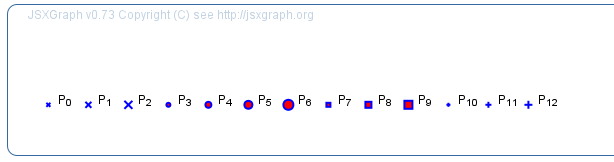
\includegraphics[width=0.4\linewidth]{images/b5.png}
\caption{All possible point styles.}\label{fig:4}
\end{figure*}
Other attributes of a point are
\bigskip
\begin{center}
\footnotesize
\begin{tabular}{lll}
\toprule
attribute name &    value   & description \\
\midrule
style                   & $0\ldots12$ & see above\\
strokeColor             & color string & \\
strokeWidth             & color string & \\
fillColor               & color string & \\
highlightStrokeColor    & color string & \\
highlightFillColor      & color string & \\
labelColor              & color string & \\
visible                 & \lstinline|true|,\lstinline|false|& point and label are visible\\
fixed                   & \lstinline|true|,\lstinline|false|& dragging possible \\
draft                   & \lstinline|true|,\lstinline|false|&  \\
trace                   & \lstinline|true|,\lstinline|false|& dragging leaves a trace\\
withLabel               & \lstinline|true|,\lstinline|false|& point has a label\\
name                    & string& label text this element\\
id                      & string&  unique id for this element\\
\bottomrule
\end{tabular}
\end{center}
If not given \lstinline|name| and \lstinline|id| are chosen automatically.

All properties beside \lstinline|id| can be changed during the life time of an object \lstinline|el|
using the method \lstinline|el.setProperty|. There are several formats possible.
\begin{lstlisting}
el.setProperty('key1:value1','key2:value2',...);
el.setProperty([key1:value1],[key2:value2],...);
el.setProperty({key1:value1, key2:value2,...});
\end{lstlisting}
